%# -*- coding: utf-8-unix -*-
%%==================================================
%% chapter01.tex for SJTU Master Thesis
%%==================================================

%\bibliographystyle{sjtu2}%[此处用于每章都生产参考文献]
\chapter{绪论}
\label{chap:intro}

\section{引言}
近年来,多机器人技术是机器人学发展的一个重要方向。这一领域研究始于20世纪80年代,最初的研究主要集中在多机器人协调,运动规划,体系结构等方面。随着相关研究的不断深入,多机器人的应用领域也越来越广,尤其是在水下,空间,未知环境探索等场合具有广阔的应用需求。总的来说,多机器人系统具有以下显著特征\supercite{蔡自兴,谭民2005多机器人系统}:
	
	(1)更广泛的任务领域。有些任务必须依靠多机器人才能完成,例如足球比赛,战术使命等。还有的任务,比如让机器人搬运一个重物,如果采用单个机器人来完成这项任务,则对单个机器人的负载、动力、能源等都有更高的要求。考虑成本以及设计复杂性,则不如采用简单机器人组成的多机器人系统来协作搬运。
	
	(2)内在的并行性。对于一些可分解的任务,多机器人系统可以将任务拆分成子任务,利用多个机器人并行完成这些子任务,从而提高任务的执行效率。例如对未知环境的建图,探索等任务。
	
	(3)更高的鲁棒性。多机器人系统中通过个体之间的通信和协作可以增加信息冗余度,避免失效点,从而提高执行任务的鲁棒性。例如,多个机器人利用摄像头采集图像对环境进行建图,若某个机器人出现故障不会对最终任务的结果产生很大影响。这样的系统具有更高的鲁棒性。
	
	(4)可以实现分布式感知与控制。对于多机器人系统中的成员进行分布式控制,这样可以针对某项任务设计合适的机器人,使得机器人的设计更具灵活性,完成有限任务的功能设计的更完善。
	
由于多机器人系统的显著优点,使得多机器人系统具有很高的潜在应用价值,应用领域非常广泛,例如:

	(1)远地作业。对于一些在高危环境或者人类无法到达环境下的任务,比如煤矿,火山口作业,或者行星探险等。机器人要能够自主完成某些任务,而人类只能适时的进行远程干预。这就需要机器人系统具有高效的任务执行能力以及较高的鲁棒性。因此对于这类系统多机器人系统能够发挥他们的优势。
	
	(2)军事行动。随着科学技术的发展以及作战环境的复杂化,信息化,多样化,单兵作战已经无法满足现代军事战争的需求。多兵种,多武器协同配合才能最大程度发挥战斗力。而随着自动化,信息化技术的发展,多机器人系统也逐渐出现在战场上,代替士兵执行危险任务或者进行更高效率的打击。
	
	(3)搜索与救援。对于灾后或者建筑物倒塌后的环境,幸存者的有效救援时间十分紧迫,并且某些空间人或者搜救犬无法到达。如果采用多机器人协作搜索,则会实现更快速更高效的搜救,为幸存者赢取宝贵的救援时间。
	
仿生一直都是人类科学创新的源泉之一。多机器人系统也不例外,受自然界中鸟群(flock)、鱼群(school)和蚁群(ant colony)等生物群体行为的影响\supercite{stilwell1993toward,theraulaz1991task,reif1999social,balch2000social,couceiro2011novel},人们越来越多的关注多机器人系统如何实现像生物群体那样的出色的集体行为能力。群机器人系统(Swarm Robotics System)便是人类模仿生物群体所进行的研究\supercite{duarte2016application,duarte2016hybrid,yu2015duration,trianni2015fundamental}。群机器人系统通过分布式控制单个机器人来模仿生物个体。通过感知周围邻居的信息,并依靠个体的局部控制实现机器人间的交互以达到某种集体行为\supercite{viksnin2016flocking,shi2012survey}。尽管群机器人系统中的个体机器人功能简单,通信能力有限,但是当多个个体协同合作时就可以完成各种更复杂的任务。而且这种系统还具有很好的可扩展性。鉴于群机器人系统中分布式控制的优势,分布式控制也在其他多机器人系统中得到广泛应用。
	
群机器人系统中典型的一类应用便是多机器人编队技术,一直以来多机器人编队技术都是研究的热点,它主要是指多机器人在运动过程中保持某种相对位置关系的控制技术\supercite{alonso2016distributed,tang2015research,yang2016behavioral}。主要分为两个部分,即多机器人编队形成和多机器人编队保持。多机器人编队形成即是使机器人由混乱随机的相对位置状态运动成具有固定的相对位置和相互作用关系的系统整体。多机器人编队保持即是通过控制与机器人间的交互保持系统内部各个机器人间的相对位置和相互作用关系不变。多机器人编队技术广泛应用在军事侦察\supercite{柳林2006多机器人系统任务分配及编队控制研究}、环境探索\supercite{renoux2015decision,abed2015multi,benavides2016multi}、灾难救援\supercite{bagosi2016ontological,liu2015multirobot,lee2016information}、协同搬运\supercite{wang2008machine,cheng2016research,fyler2015distributed}等任务。在军事侦察任务中,多无人机或无人车组成编队对某一环境进行侦察,不但可以更快速更广范围的侦察环境,而且还可以通过不同机器人上配置不同传感器实现多种信息融合,保证侦察效果与精度。在环境探索和灾难救援任务中,多机器人通过实时变换和优化编队队形来更有效率的探索某一环境。同样可以通过在编队中不同位置的机器人装配不同类型的传感器,从而可以最大发挥各种传感器在不同环境探索中的优势。在协同搬运任务中,多机器人根据重物的特点形成最有效的队形,通过同步运动搬运重物。这样有助于分解重物的重量,减小单个机器人的负载,从而可以搬运单个机器人无法搬运的重物。

尽管多机器人编队系统相对于单个机器人能够高效率,高质量的完成某些任务,但是可以看到,多机器人系统大多工作在大范围,更复杂的环境中。由于工作环境中存在诸多的不确定性,编队中个别机器人出现故障的情况难以避免。尽管多机器人系统具有更高的鲁棒性和冗余性,但是如果任由机器人发生故障而失效,就可能会降低工作效率,影响任务完成质量。对于编队中某些关键位置机器人的失效可能会导致编队分裂,机器人信息无法传播,从而使得任务失败。或者在重物搬运过程中,某个机器人的失效导致重物重心不稳,或者机器人负载不均衡,不仅任务失败甚至还可能对其他机器人造成损坏,带来更大的损失。因此针对这一问题,我们需要多机器人编队系统具有自修复能力,能够在编队中机器人出现缺失的情况下自主恢复原来的编队队形以及系统性能。

\section{多机器人系统自修复研究概述}
随着研究的不断深入,在多机器人以及多智能体网络领域涌现了大批的自修复算法。这些自修复算法大致可以分为以下三类\supercite{张飞2010}:

\subsection{直接自修复算法}
直接自修复算法是指当网络中出现节点丢失时,采用直接指定某一节点去修复缺失节点的方式。在文献\parencite{corke2004autonomous}中,作者设计了如何创建和保持多传感器网络特定拓扑结构以及通信连接的节点分配和修复算法。作者利用无人机对整个传感器网络进行监控和调度。直升机可以和所有节点通信并构建整个网络拓扑连接,如图\ref{fig:直接自修复-无人机}所示。当直升机发现某个节点不在拓扑范围之内,直升机会重新分配此节点。如果发现网络拓扑连接某处出现断裂,则无人机会调整拓扑内部节点进行修复。在这一应用中,直升机起到一个监控中心、决策中心和调度中心的作用,属于集中式控制。重要适用于静态的拓扑控制,并且对无人机端的数据处理能力和稳定性要求较高。
%\begin{figure*}[!htbp]
%	\centering
%	\subfigure[]{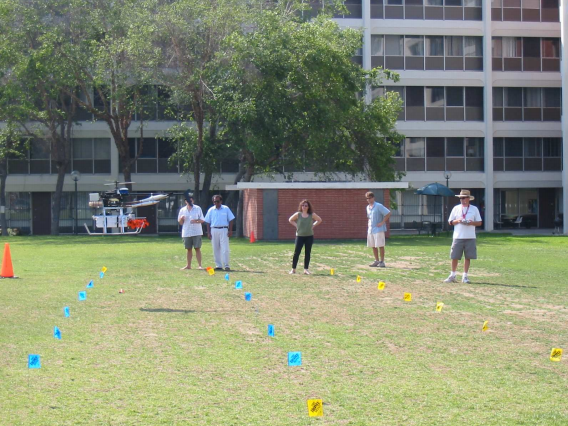
\includegraphics[width=0.3\textwidth]{figure1-1.1.png}}
%	\hspace{1cm}
%	\subfigure[]{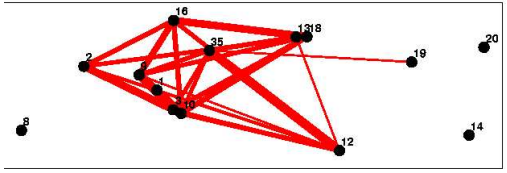
\includegraphics[width=0.3\textwidth]{figure1-1.2.png}}

%	\subfigure[]{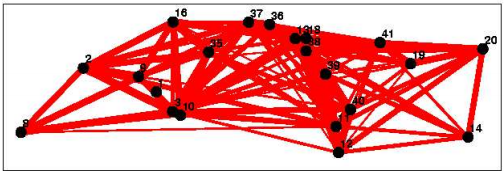
\includegraphics[width=0.3\textwidth]{figure1-1.3.png}}		
%	\bicaption[fig:SRR]{这里将出现在插图索引中}{中文题图}{Fig}{English caption}
%\end{figure*}
\begin{figure*}[!htbp]
	\begin{multicols}{2}
		
		\begin{center}
			\subfigure[无人机集中式控制拓扑网络]{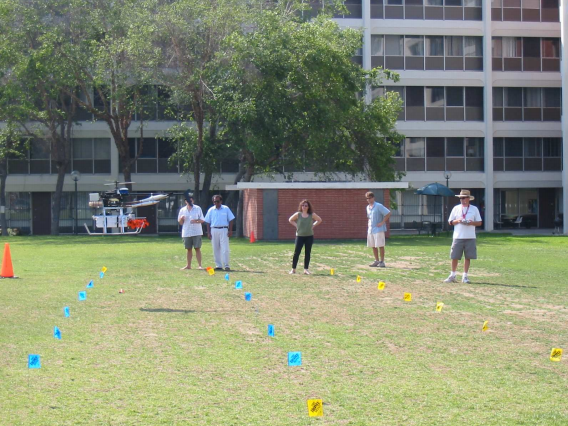
\includegraphics[width=6cm,height=4.8cm]{figure1-1.1.png}}
		\end{center}
		\begin{center}
			\subfigure[修复前的拓扑网络]{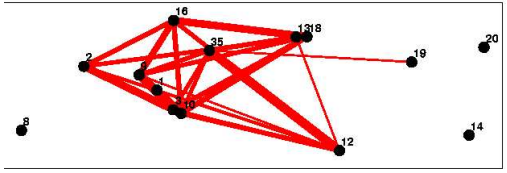
\includegraphics[width=5cm,height=1.7cm]{figure1-1.2.png}}
		\end{center}
		\begin{center}
			\subfigure[修复后的拓扑网络]{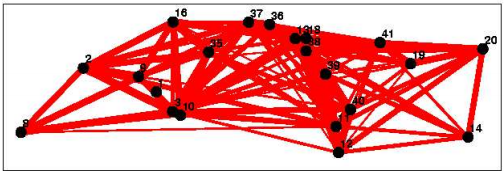
\includegraphics[width=5cm,height=1.7cm]{figure1-1.3.png}}
		\end{center}
	\end{multicols}
	\bicaption[fig:直接自修复-无人机]{利用无人机进行集中式控制拓扑网络的直接自修复算法}{利用无人机机进行集中式控制拓扑网络的直接自修复算法}{Fig}{Autonomous deployment and repair of a sendor network using an unmanned aerial vehicle}
\end{figure*}

文献\parencite{Auto-holeDetection}中针对传感器网络覆盖问题进行了自修复的研究。文中主要针对网络覆盖中的空缺进行探测并修复。在算法执行过程中每个传感器节点与其他节点交换信息,多次交换信息后每个节点可以获得一个以它自身为中心的x-hop的邻居列表。即每一个节点能够获得拓扑网络中所有其他节点的信息,并计算出每个节点距离自己的跳数。如果出现空洞,则节点会根据自己的邻居列表选出一条修复路径,然后从所有的路径中选择一条效率最高的路径执行自修复。该算法需要每个节点都能够获得其他节点的信息,通信量比较大,且对每个节点的存储空间有所要求。若实现大规模节点的自修复则算法的时间和空间复杂度比较大,实现效率较低。

文献\parencite{Zhang2006Motion}针对多机器人编队网络的运动同步性进行自修复。当多机器人编队网络中出现机器人故障或者通信失效时,可能会影响整个网络的运动同步性。此时文中算法采用临时扩大机器人通信范围的方式,使得编队中所有机器人能够共享信息,从而直接选出合适的修复机器人进行自修复。修复过程如图\ref{fig:直接自修复-同步性}所示。
\begin{figure*}[!htbp]
	\begin{multicols}{2}
		\begin{center}
			\subfigure[]{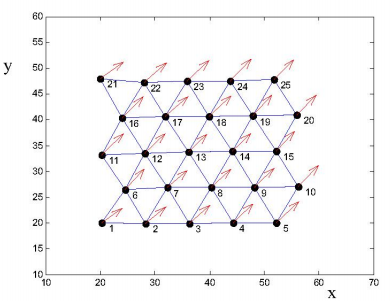
\includegraphics[width=6cm, height=4cm]{figure1-2.a.png}}
		\end{center}
		\begin{center}
			\subfigure[]{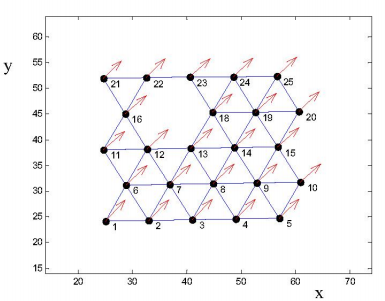
\includegraphics[width=6cm,height=4cm]{figure1-2.b.png}}
		\end{center}
		\begin{center}
			\subfigure[]{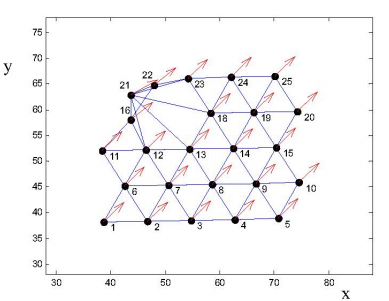
\includegraphics[width=6cm,height=4cm]{figure1-2.c.png}}
		\end{center}
		\begin{center}
			\subfigure[]{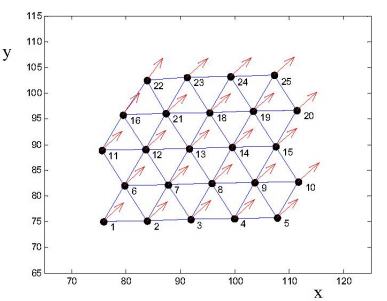
\includegraphics[width=6cm,height=4cm]{figure1-2.d.png}}
		\end{center}
	\end{multicols}
	\bicaption[fig:直接自修复-同步性]{多机器人编队网络运动同步性直接自修复}{多机器人编队网络运动同步性直接自修复}{Fig}{Directly self-healing for multi-robot formation motion synchronization.}	
\end{figure*}
由于出现机器人缺失后需要临时扩大机器人的通信范围,因此,算法不能算是完全分布式。并且多机器人的编队规模要收到传感器的最大通信距离的限制,不可能实现大规模机器人的编队控制,并且同样通信时间以及复杂度要随着编队规模的扩大呈指数型增长。

\subsection{密度自修复算法}
密度自修复算法主要应用在大量机器人进行自组装,形态生成或者区域覆盖等任务中。系统中的节点能够感知自身所处位置的密度,以此作为依据执行自修复算法,最终能够能够根据系统要求取得合理分布。文献\parencite{arbuckle2010self}中,作者仿照生物学纳米分子间信息交流的方式,研究了多智能体自主形态生成问题。在系统中已知一个几何形状,然后解析出几何形状的边集合,节点的有序集合。通过大量统一结构、统一编程的微小机器人执行分布式的形态生成算法可以构建出任意指定的形状。并且算法具有一定的容错机制,能够针对机器人失效,进行自修复。如图\ref{fig:密度自修复-形态生成}所示。
\begin{figure}[!htbp]
	\centering
	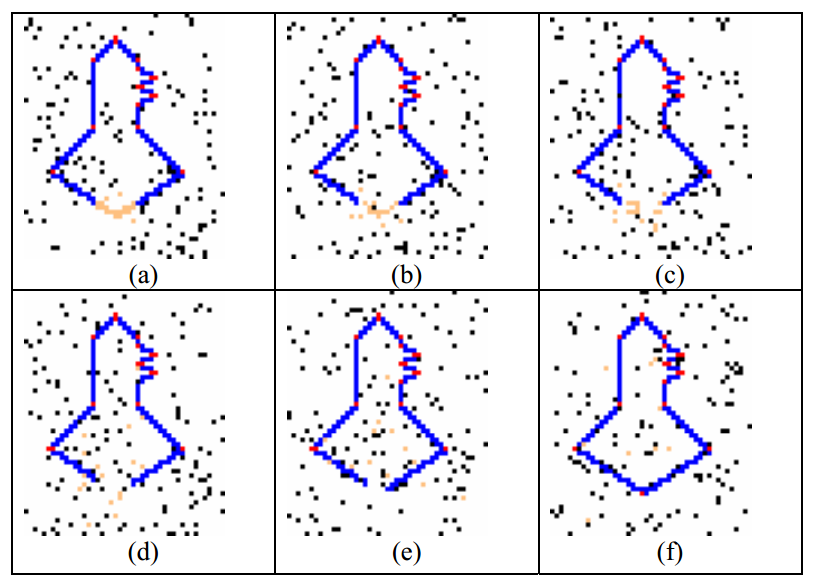
\includegraphics[width=10cm,height=6cm]{figure1-3.png}
	\bicaption[fig:密度自修复-形态生成]{形态生成过程中机器人失效后的自修复}{形态生成过程中机器人失效后的自修复\supercite{arbuckle2010self}}{Fig}{The structure recovers from the damage and self-repairs\supercite{arbuckle2010self}}
\end{figure}
然而此算法的自修复过程具有一定的负面效应。即当机器人数量比较多,信息共享不完全时可能在系统中复制出两个完全一样的形状。

在文献\parencite{derbakova2011decentralized}中,作者研究了群机器人有效覆盖特定区域的算法。该算法能够实现群机器人针对某一区域的覆盖,并能对覆盖失效的情况进行自修复。系统中存在一个网关,负责所有机器人之间通信的中转,每个机器人通过与邻居通信间接与网关链接。在已知感兴趣区域的形状之后,机器人根据自身位置,结合密度信息执行分散算法,最终能够均匀覆盖该区域。并且在区域内某些机器人被移除后,系统能够自动感知缺失,并通过网关进行路径规划,调度其他机器人重新均匀覆盖此区域。如图\ref{fig:密度自修复-区域覆盖}所示。
\begin{figure*}[!htbp]
	\centering
	\begin{tabular}{cccc}
			\subfigure[]{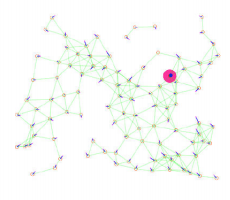
\includegraphics[width=3cm,height=4cm]{figure1-4.a.png}} &
			\subfigure[]{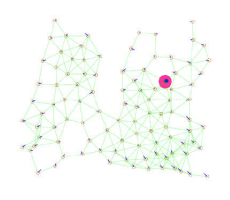
\includegraphics[width=3cm,height=4cm]{figure1-4.b.png}} &
			\subfigure[]{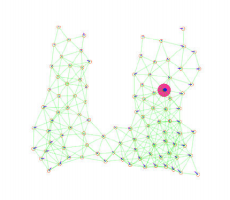
\includegraphics[width=3cm,height=4cm]{figure1-4.c.png}} &
			\subfigure[]{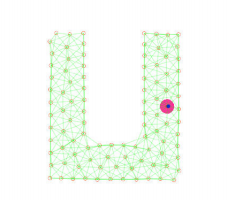
\includegraphics[width=3cm,height=4cm]{figure1-4.d.png}} \\
			\subfigure[]{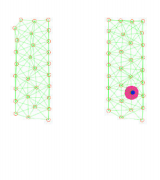
\includegraphics[width=3cm,height=4cm]{figure1-4.e.png}} &
			\subfigure[]{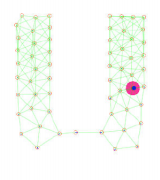
\includegraphics[width=3cm,height=4cm]{figure1-4.f.png}} & 
			\subfigure[]{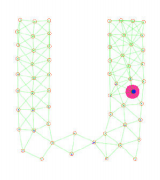
\includegraphics[width=3cm,height=4cm]{figure1-4.g.png}} &
			\subfigure[]{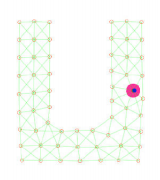
\includegraphics[width=3cm,height=4cm]{figure1-4.h.png}} \\
	\end{tabular}
	\bicaption[fig:密度自修复-区域覆盖]{多移动机器人区域覆盖网络连接自修复算法}{多移动机器人区域覆盖网络连接自修复算法}{Fig}{Coverage and repair algorithm for multi-robot systems}
\end{figure*}
\subsection{递归自修复算法}
递归自修复算法利用节点或机器人之间局部交互和网络拓扑切换实现自修复。在文献\parencite{abbasi2009movement}中Abbassi等人针对无线传感器执行器网络(Wireless Sensor and Actor Networks, WSANs)中节点失效影响网络连通性的问题,提出了DARA(Distributed Actor Recovery Algorithm)算法。DARA算法针对不同的网络拓扑分为DARA-1C和DARA-2C两个版本。DARA-1C算法用于维持和修复网络的一阶连通性。算法通过心跳机制\supercite{王海龙2009基于实时以太网的心跳协议}检测网络中的节点丢失。当节点出现丢失时从丢失节点的邻居中根据节点的度、离缺失节点的距离大小、自身ID号等条件选取最佳候选修复节点。网络中每个节点维持二跳邻居信息,主要针对网络中割点(cut-vertex)丢失导致网络分裂成两个或多个部分的问题进行修复。如图\ref{fig:递归自修复-DARA-1C}所示。
\begin{figure*}[!htbp]
	\centering
	\begin{tabular}{ccc}
		\subfigure[]{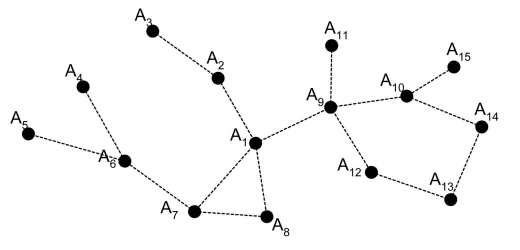
\includegraphics[width=5cm,height=3cm]{figure1-5.a.png}}
		\subfigure[]{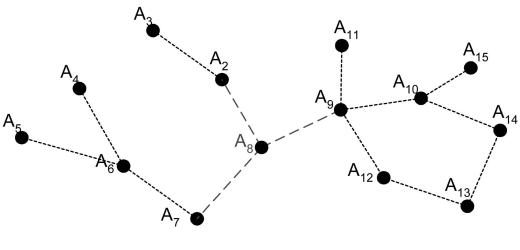
\includegraphics[width=5cm,height=3cm]{figure1-5.b.png}}
		\subfigure[]{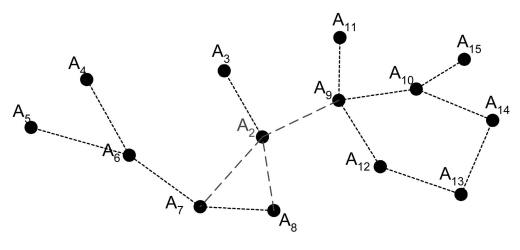
\includegraphics[width=5cm,height=3cm]{figure1-5.c.png}}
	\end{tabular}
	\bicaption[fig:递归自修复-DARA-1C]{使用DARA-1C算法实现传感器网络连接自修复}{使用DARA-1C算法实现传感器网络连接自修复}{Fig}{Using DARA-1C to repair the connectivity of WSANs}
\end{figure*}

DARA-2C算法目的是维持网络的2阶连通性。可以实现网络外围节点丢失的自修复。算法的实现方式与DARA-1C类似,但主要是针对网络边缘节点进行自修复,目的是防止出现割点(cut-vertex)。修复算法只考虑是否维持2阶连通性。修复过程如图\ref{fig:递归自修复-DARA-2C}所示。
\begin{figure}[!htbp]
	\centering
	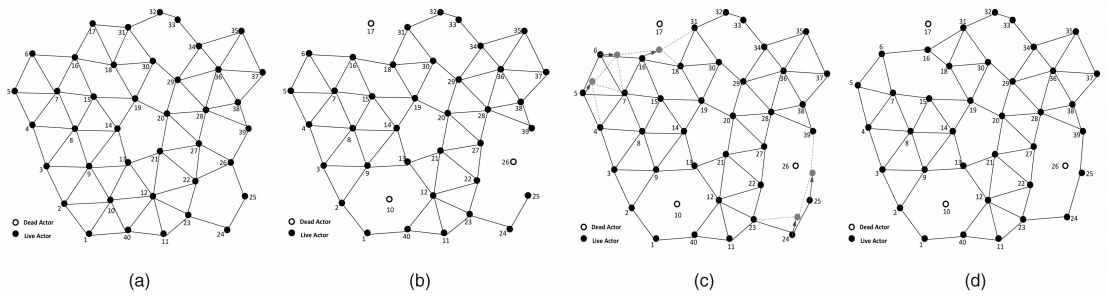
\includegraphics[width=15cm,height=4cm]{figure1-6.png}
	\bicaption[fig:递归自修复-DARA-2C]{使用DARA-2C算法实现传感器网络2阶连通性自修复}{使用DARA-2C算法实现传感器网络2阶连通性自修复}{Fig}{Using DARA-2C to repair 2-connectivity of WSANs}
\end{figure}

在文献\parencite{younis2010localized}中,同样针对传感器网络连通性问题,Younis等人提出了RIM(Recovery through Inward Motion)自修复算法。该算法主要是在节点出现缺失之后,缺失节点的所有邻居节点全部向缺失节点的位置移动,直至重新建立连接。缺失节点的邻居节点移动后若如出现新的空缺则由其邻居继续执行RIM算法进行自修复,直至整个网络保持连通。如图\ref{fig:递归自修复-RIM}所示。该算法只考虑网络的连通性,不考虑拓扑结构的变化。
\begin{figure}
	\centering
	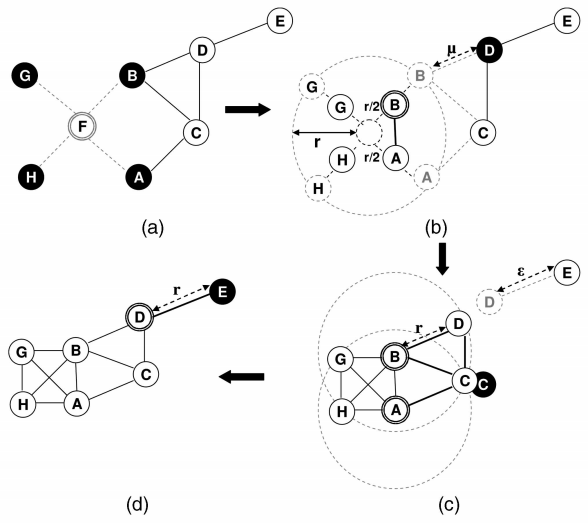
\includegraphics[width=9cm,height=8cm]{figure1-7.png}
	\bicaption[fig:递归自修复-RIM]{RIM算法自修复过程}{RIM算法自修复过程}{Fig}{The self-healing process of RIM algorithm}
\end{figure}

前人关于自修复的算法几乎都是针对网络的联通性。然而类似于多机器人协同搬运这样的任务,需要多机器人能够保持特定的队形并且对编队的运动同步性要求较高。多机器人运动同步是指多个机器人通过局部交互最终达到运动速度同步\supercite{张飞2008移动机器人覆盖问题的研究,Zhang2006Motion}。显然上述算法都无法适用于针对多机器人编队运动同步性的自修复。因此如何设计一种性能良好的针对多机器人编队网络运动同步性的自修复算法是值得思考和亟需解决的问题\footnote{本文同步性皆指的是运动同步性。}。

\section{本文研究内容及组织框架}
本文针对多机器人编队网络中存在机器人缺失,从而导致整个编队运动同步性下降的问题,提出了一种同步性改善全局最优的分布式自修复算法。该算法能够实现同步性改善全局最优,通过在编队网络中构建稳定的梯度分布可以找到一条实现同步性改善全局最优的修复路径,并且该修复路径包含修复机器人个数最少,机器人运动的总距离最短。针对本文算法,不仅利用仿真验证了算法的理论可行性和有效性,而且还设计了包括多机器人空间定位系统,通信系统,运动控制系统在内的自修复实验平台。在此平台下开展了实验,验证了算法的现实可行性和可操作性。

本文主要贡献如下:\\
\indent 1) 提出了一种分布式的多机器人编队自修复算法。该算法在编队中出现机器人缺失后不仅修复了编队队形还能够实现同步性改善全局最优。\\
\indent 2) 在本文算法中引入梯度,并设计了一中新的梯度扩散与更新机制,从而实现同步性改善全局最优的同时保证修复路径最短,修复机器人个数最少。\\
\indent 3) 设计了仿真验证算法在同步性改善、修复机器人个数、修复机器人运动距离等指标的考量。\\
\indent 4) 设计了多机器人编队自修复实验平台。平台包括基于Vicon的多功能可扩展的空间定位系统、机器人个体运动控制系统和远程控制系统。

本文各章节简介如下:\\
\indent 第一章,介绍多机器人编队自修复研究的背景及前人工作,引出本文所要解决的问题。\\
\indent 第二章,分析了编队网络拓扑模型与机器人个体运动模型,介绍编队同步性与网络拓扑的关系。\\
\indent 第三章,详细介绍了本文提出的同步性改善全局最优自修复算法,并分析算法的相关性能指标。\\
\indent 第四章,设计了仿真,通过对比分析验证了本文算法的可行性与有效性及相比前人工作的优势。\\
\indent 第五章,设计了用于实现多机器人编队自修复算法的实验平台,包括定位系统,机器人个体控制与通信系统,远程控制系统。并在此平台下进行实验,验证本文算法的可行性和有效性\\
\indent 第六章,全文工作总结及未来工作展望。

